\documentclass[a5paper, 10pt]{article}

% Текст
\usepackage[utf8]{inputenc} % UTF-8 кодировка
\usepackage[russian]{babel} % Русский язык
\usepackage{indentfirst} % красная строка в первом параграфе в главе
% Отображение страниц
\usepackage{geometry} % размеры листа и отступов
\usepackage{listings}
\usepackage{color}

\geometry{
	left=12mm,
	top=25mm,
	right=15mm,
	bottom=17mm,
	marginparsep=0mm,
	marginparwidth=0mm,
	headheight=10mm,
	headsep=7mm,
	nofoot}
\usepackage{afterpage,fancyhdr} % настройка колонтитулов
\pagestyle{fancy}
\fancypagestyle{style}{ % создание нового стиля style
	\fancyhf{} % очистка колонтитулов
	\fancyhead[LO, RE]{Лабораторная работа № 3 } % название документа наверху
	\fancyhead[RO, LE]{Задачи 1207, 1322, 1444} % название section наверху
	\fancyfoot[RO, LE]{\thepage} % номер страницы справа внизу на нечетных и слева внизу на четных
	\renewcommand{\headrulewidth}{0.25pt} % толщина линии сверху
	\renewcommand{\footrulewidth}{0pt} % толцина линии снизу
}
\fancypagestyle{plain}{ % создание нового стиля plain -- полностью пустого
	\fancyhf{}
	\renewcommand{\headrulewidth}{0pt}
}
\fancypagestyle{title}{ % создание нового стиля title -- для титульной страницы
	\fancyhf{}
	\fancyhead[C]{{\footnotesize
			Министерство образования и науки Российской Федерации\\
			Федеральное государственное автономное образовательное учреждение высшего образования
	}}
	\fancyfoot[C]{{\large 
			Санкт-Петербург, 2024
	}}
	\renewcommand{\headrulewidth}{0pt}
}

% Математика
\usepackage{amsmath, amsfonts, amssymb, amsthm} % Набор пакетов для математических текстов
%\usepackage{dmvnbase} % мехматовский пакет latex-сокращений
\usepackage{cancel} % зачеркивание для сокращений
% Рисунки и фигуры
\usepackage[pdftex]{graphicx} % вставка рисунков
\usepackage{wrapfig, subcaption} % вставка фигур, обтекая текст
\usepackage{caption} % для настройки подписей
\captionsetup{figurewithin=none,labelsep=period, font={small,it}} % настройка подписей к рисункам
% Рисование
\usepackage{tikz} % рисование
\usepackage{circuitikz}
\usepackage{pgfplots} % графики
% Таблицы
\usepackage{multirow} % объединение строк
\usepackage{multicol} % объединение столбцов
% Остальное
\usepackage[unicode, pdftex]{hyperref} % гиперссылки
\usepackage{enumitem} % нормальное оформление списков
\setlist{itemsep=0.15cm,topsep=0.15cm,parsep=1pt} % настройки списков
% Теоремы, леммы, определения...
\theoremstyle{definition}
\newtheorem{Def}{Определение}
\newtheorem*{Axiom}{Аксиома}
\theoremstyle{plain}
\newtheorem{Th}{Теорема}
\newtheorem{Lem}{Лемма}
\newtheorem{Cor}{Следствие}
\newtheorem{Ex}{Пример}
\theoremstyle{remark}
\newtheorem*{Note}{Замечание}
\newtheorem*{Solution}{Решение}
\newtheorem*{Proof}{Доказательство}
% Свои команды
\newcommand{\comb}[1]{\left[\hspace{-4pt}\begin{array}{l}#1\end{array}\right.\hspace{-5pt} } % совокупность уравнений
% Титульный лист
\usepackage{csvsimple-l3}
\newcommand*{\titlePage}{
	\thispagestyle{title}
	\begingroup
	\begin{center}
		%		{\footnotesize
			%			Министерство образования и науки Российской Федерации\\
			%			Федеральное государственное автономное образовательное учреждение высшего образования
			%		}
		%		
		\vspace*{6ex}
		
		{\small
			САНКТ-ПЕТЕРБУРГСКИЙ НАЦИОНАЛЬНЫЙ ИССЛЕДОВАТЕЛЬСКИЙ УНИВЕРСИТЕТ ИТМО	
		}
		
		\vspace*{2ex}
		
		{\normalsize
			Факультет систем управления и робототехники
		}
		
		\vspace*{15ex}
		
		{\Large \bfseries 
			Лабораторная работа № 3
		}
\vspace*{2ex}
	{\Large \bfseries 
			
"Задачи 1207, 1322, 1444"
		}
\vspace*{2ex}
		
		{\normalsize
			по дисциплине Алгоритмы и структуры данных
		}

	\end{center}
	\vspace*{20ex}
	\begin{flushright}
		{\large 
			\underline{Выполнила}: студентка гр. \textbf{R3238}\\
                             поток \textbf{2.1}\\
			\begin{flushright}
				\textbf{Нечаева А. А.}\\
			\end{flushright}
		}
		
		\vspace*{5ex}
		
		{\large 
			\underline{Преподаватель}: \textit{Тропченко Андрей Александрович}
		}
	\end{flushright}	
	\newpage
	\setcounter{page}{1}
	\endgroup}

\begin{document}
	\titlePage
	\pagestyle{style}

\lstset{ %
language=C,                 % выбор языка для подсветки (здесь это С)
basicstyle=\small\sffamily, % размер и начертание шрифта для подсветки кода
numbers=left,               % где поставить нумерацию строк (слева\справа)
numberstyle=\tiny,           % размер шрифта для номеров строк
stepnumber=1,                   % размер шага между двумя номерами строк
numbersep=5pt,                % как далеко отстоят номера строк от подсвечиваемого кода
backgroundcolor=\color{white}, % цвет фона подсветки - используем \usepackage{color}
showspaces=false,            % показывать или нет пробелы специальными отступами
showstringspaces=false,      % показывать или нет пробелы в строках
showtabs=false,             % показывать или нет табуляцию в строках
frame=single,              % рисовать рамку вокруг кода
tabsize=2,                 % размер табуляции по умолчанию равен 2 пробелам
captionpos=t,              % позиция заголовка вверху [t] или внизу [b] 
breaklines=true,           % автоматически переносить строки (да\нет)
breakatwhitespace=false, % переносить строки только если есть пробел
escapeinside={\%*}{*)}   % если нужно добавить комментарии в коде
}



\newpage
\section{Цель}
Разработать и реализовать алгоритмы для решения задач 1207, 1322 и 1444.


\section{Задача 1207}

\begin{figure}[h]
\center{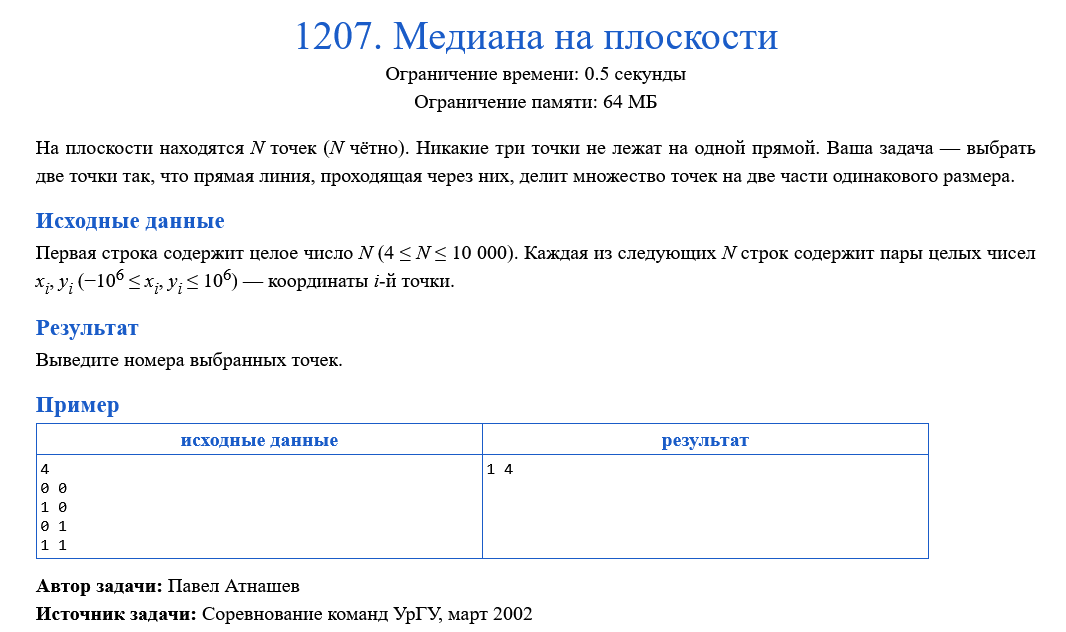
\includegraphics[width=0.9\linewidth]{pic/task_1207.png}}
\caption{Условие задачи 1207.}
\end{figure}

\subsection{Основная идея}
Задача сводится к поиску максимальной суммы подпоследовательности последовательности $p_i$.

\subsection{Краткое описание алгоритма}
\textbf{1. Входные данные:} первая строка содержит целое число $N\, (4 \leq N \leq 10000)$. Каждая из следующих $N$ строк содержит пары целых чисел $x_i, y_i \, (-10^6 \leq x_i, y_i \leq 10^6)$-- координаты $i$-й точки. \\
\textbf{2.} Для разделения плоскости на 2 части необходимо найти точку, которая расположена левее всех остальных. \\
\textbf{3.} Далее определим угол прямой, проведенной до каждой из оставшихся точек и отсортируем точки по величине угла. \\
\textbf{4.} Теперь мы можем определить точку, через которую проходит прямая, разделяющая точки на плоскости пополам. \\
\textbf{5.} Выходные данные: порядковые номера 2-х точек, прямая через которые разделитт все точки плоскости на 2 равные половины.

\subsection{Листинг}

\begin{center}
\begin{lstlisting}[label=some-code,caption={Исходный код для 1207}]
#include <iostream>
#include <cmath>

#define PI 3.14159265358979323846

// new struct for points, it keeps x, y, number of the point and angle
struct point_struct {
    int x;
    int y;
    double angle;
    int num;
};

point_struct data[10000];

bool compare(point_struct a, point_struct b) {
    return a.angle < b.angle;
}

void quick_sort(int left, int right){
    int i = left;
    int j = right;

    point_struct median = data[(left + right) / 2];

    while (i <= j) {
        while (compare(data[i], median)) {
            ++i;
        }
        while (compare(median, data[j])) {
            --j;
        }
        if (i <= j) {
            std::swap(data[i], data[j]);
            ++i;
            --j;
        }
    }
    if (i < right) {
        quick_sort(i, right);
    }
    if (left < j) {
        quick_sort(left, j);
    }
};

int main() {
    int n;
    std::cin >> n;

    int first_x = 1000000;
    int first_id = 0;

    for (int i = 0; i < n; ++i) {
        int p_x;
        int p_y;

        std::cin >> p_x >> p_y;

        if (p_x < first_x) {
            first_id = i;
            first_x = p_x;
        }

        data[i].x = p_x;
        data[i].y = p_y;
        data[i].num = i;
    }

    // here we analyze the angles
    for (int i = 0; i < n; ++i) {
        if (data[i].num == first_id) {
            data[i].angle = -360;
        } else {
            if (data[i].x == data[first_id].x) {
                if (data[i].y > data[first_id].y) {
                    data[i].angle = 90;
                } else {
                    data[i].angle = -90;
                }
            } else {
                data[i].angle = atan((double) (data[i].y - data[first_id].y) / (data[i].x - data[first_id].x)) * 180.0 / PI;
            }
        }
    }

    quick_sort(0, n - 1);

    std::cout << first_id + 1 << " " << data[n / 2].num + 1 << std::endl;

    return 0;
}

\end{lstlisting}
\end{center}

\subsection{Результат}
\begin{figure}[h]
\center{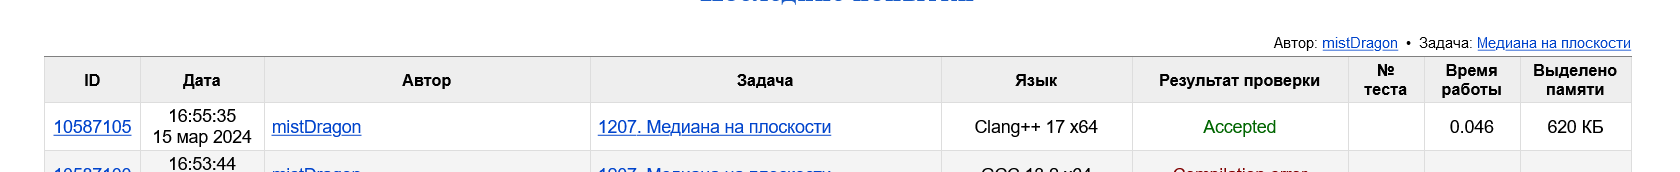
\includegraphics[width=0.9\linewidth]{pic/screen_1207.png}}
\caption{Результат отправки задачи 1207.}
\end{figure}


\newpage

\section{Задача 1322}

\begin{figure}[h]
\center{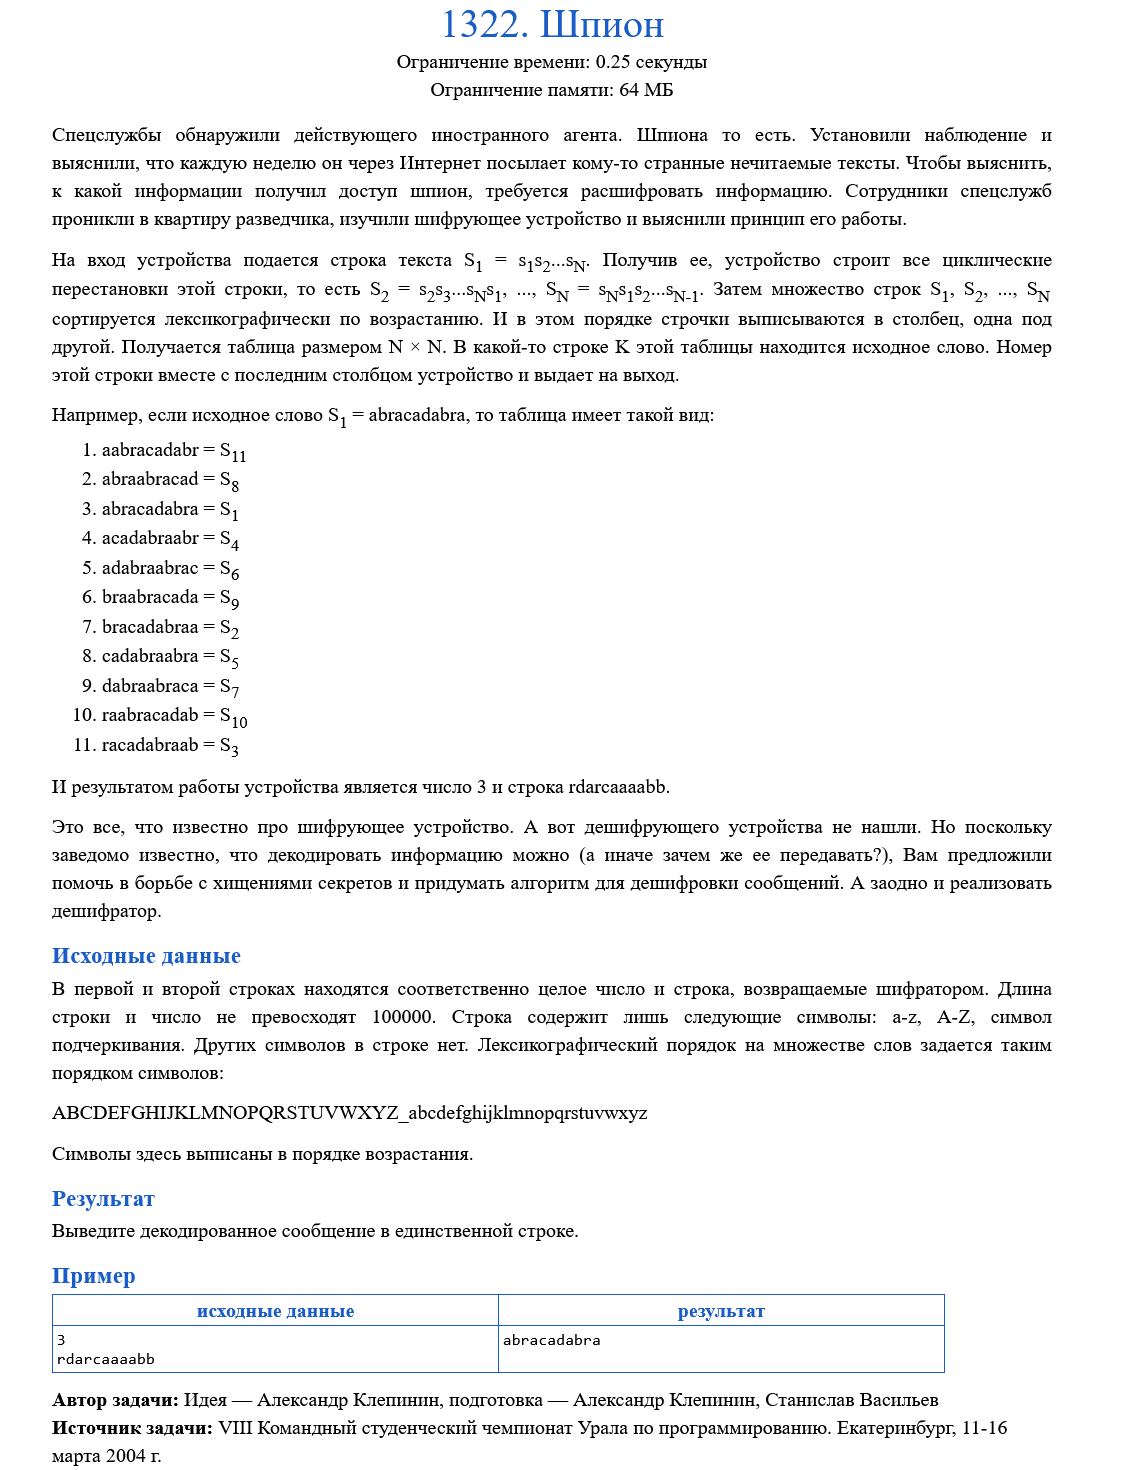
\includegraphics[width=0.773\linewidth]{pic/task_1322.png}}
\caption{Условие задачи 1322.}
\end{figure}

\subsection{Основная идея}

Задача сводится к работе с \textbf{преобразованием Барроуза--Уилера}, в нашем случае необходимо выполнить обратное преобразование.

\subsection{Краткое описание алгоритма}
\textbf{1. Входные данные:} целое число $s \, \, (s \leq 100000) $ и строка $str$. \\
\textbf{2.} Последовательно восстанавливаем строку. Пусть изначально известно, каким по порядку является приписанный в начало символ (его порядок в столбце)\\
\textbf{3.} Из предыдущего шага известно, какое место занимала строка без первого символа (i-ое).\\
\textbf{4.} Несложно заметить, что при выполнении такой операции строка с номером $i$ всегда будет перемещаться на позицию с номером $j$.\\
\textbf{5. Выходные данные:} строка.

\subsection{Листинг}

\begin{center}
\begin{lstlisting}[label=some-code,caption={Исходный код для 1322}]
#include <iostream>


const int maximum_n = 100000;

std::pair<char, int> data[maximum_n];

bool comparator(std::pair<char, int> first, std::pair<char, int> second) {
    return (first.first != second.first) ? first.first < second.first : first.second < second.second;
}

//sort in lexicographic order (quick sort)
void sorter(int left, int right) {
    int i = left;
    int j = right;

    std::pair<char, int> cur = data[(left + right) / 2];

    while (i <= j) {
        while (comparator(data[i], cur)) {
            ++i;
        }
        while (comparator(cur, data[j])) {
            --j;
        }

        if (i <= j) {
            std::swap(data[i++], data[j--]);
        }
    }

    if (i < right) sorter(i, right);

    if (j > left) sorter(left, j);

}

int main() {
    int s;
    std::string str;

    std::cin >> s >> str;

    int symbols_counter = str.length();

    for (int i = 0; i < symbols_counter; ++i) {
        data[i].first = str[i];
        data[i].second = i;
    }

    sorter(0, symbols_counter - 1);

    int result[symbols_counter];

    for (int i = 0; i < symbols_counter; ++i) {
        result[i] = data[i].second;
    }

    int current = s - 1;

    for (int i = 0; i < symbols_counter; ++i) {
        std::cout << data[current].first;
        current = result[current];
    }

    return 0;
}

\end{lstlisting}
\end{center}

\subsection{Результат}

\begin{figure}[h]
\center{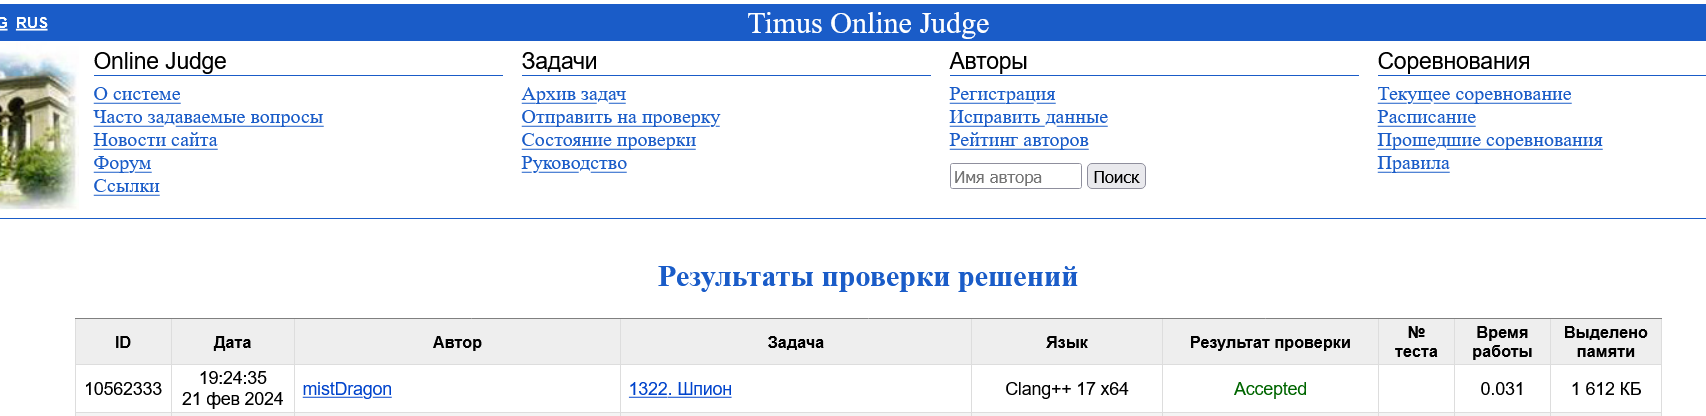
\includegraphics[width=0.9\linewidth]{pic/screen_1322.png}}
\caption{Результат отправки задачи 1322.}
\end{figure}



\newpage
\section{Задача 1444}

\begin{figure}[h]
\center{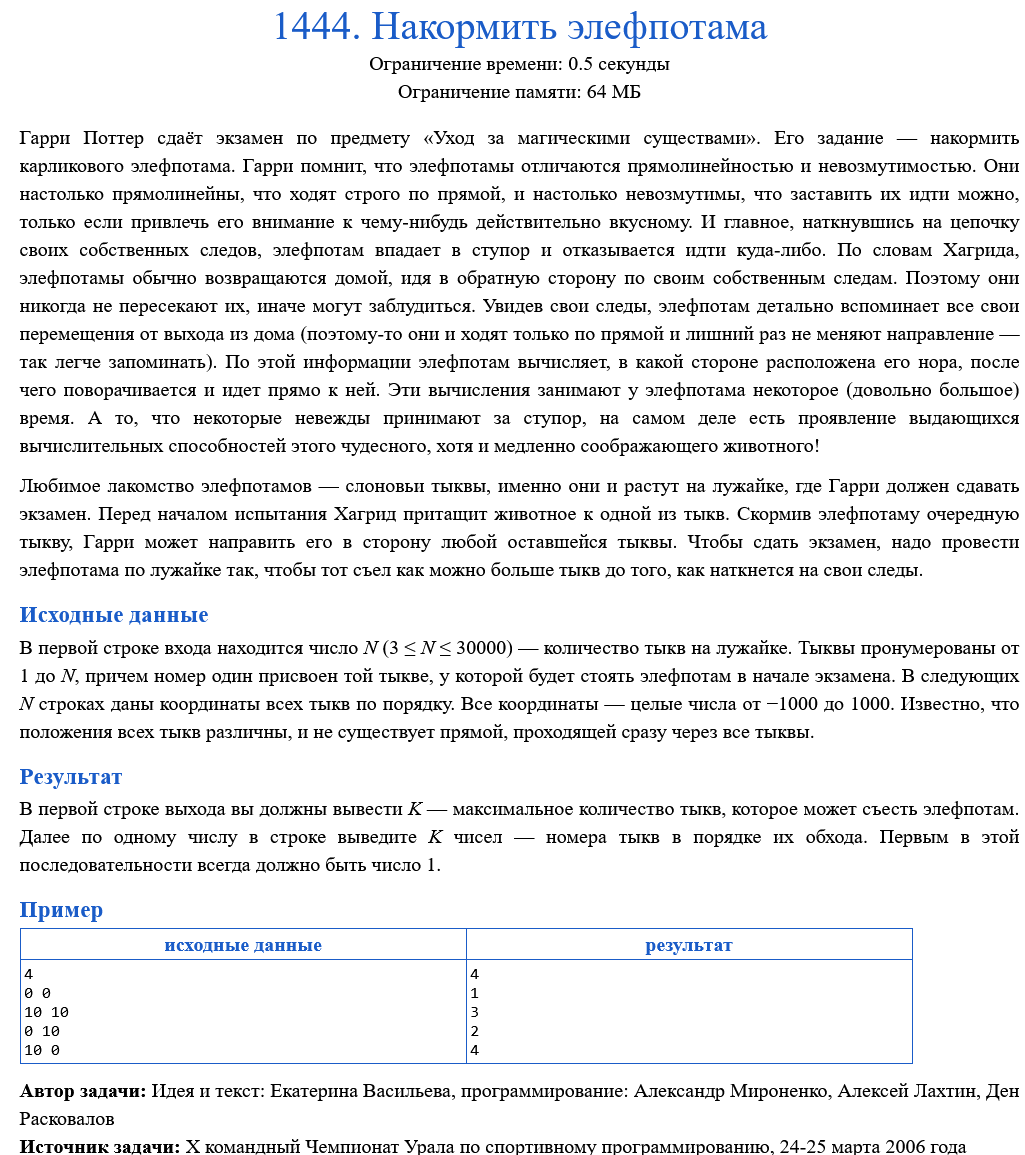
\includegraphics[width=0.9\linewidth]{pic/task_1444.png}}
\caption{Условие задачи 1444.}
\end{figure}

\subsection{Основная идея}
Задача сводится к поиску максимальной суммы подпоследовательности последовательности $p_i$.

\subsection{Краткое описание алгоритма}
\textbf{1. Входные данные:} \\
\textbf{2.} \\
\textbf{3.} \\
\textbf{4.} \\
\textbf{5. Выходные данные:} 

\subsection{Листинг}

\begin{center}
\begin{lstlisting}[label=some-code,caption={Исходный код для 1444}]
#include <iostream>


\end{lstlisting}
\end{center}

\subsection{Результат}
%\begin{figure}[h]
%\center{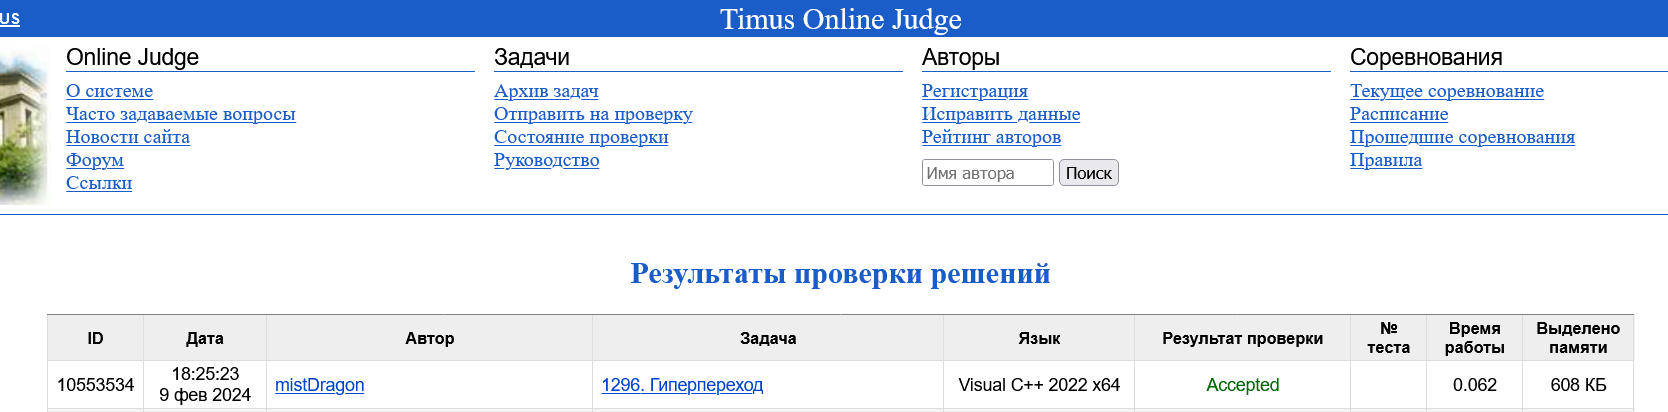
\includegraphics[width=0.9\linewidth]{pic/screen_1296.png}}
%\caption{Результат отправки задачи 1296.}
%\end{figure}


\newpage



\newpage
\section{Вывод по работе}
В ходе выполнения данной лабораторной работы были реализованы алгоритмы для решения задач $1207$, $1322$ и $1444$. 
\end{document}













